\section{Shallow Water Equations and the Serre-Green-Nagdhi Model}

The shallow water equations are a set of equations that govern the flow of a viscous, Newtonian fluid in a domain where the horizontal length scale is much larger than the veritcal length scale. Some examples of such flows are ocean waves, tsunamis, and debris slides. The shallow water model is a hyperbolic system of PDEs presented as
\begin{align}
    \begin{cases}
        \frac{\partial h}{\partial t} + \nabla \cdot (h \textbf{u}) = 0 \\
        \frac{\partial h \textbf{u}}{\partial t} + \nabla \cdot (h \textbf{u} \otimes \textbf{u}) = 0 \\
    \end{cases}
\end{align}
The diagram and reference frame for the shallow water equations are shown in \ref{fig_swe}.

\begin{figure}
    \centering
    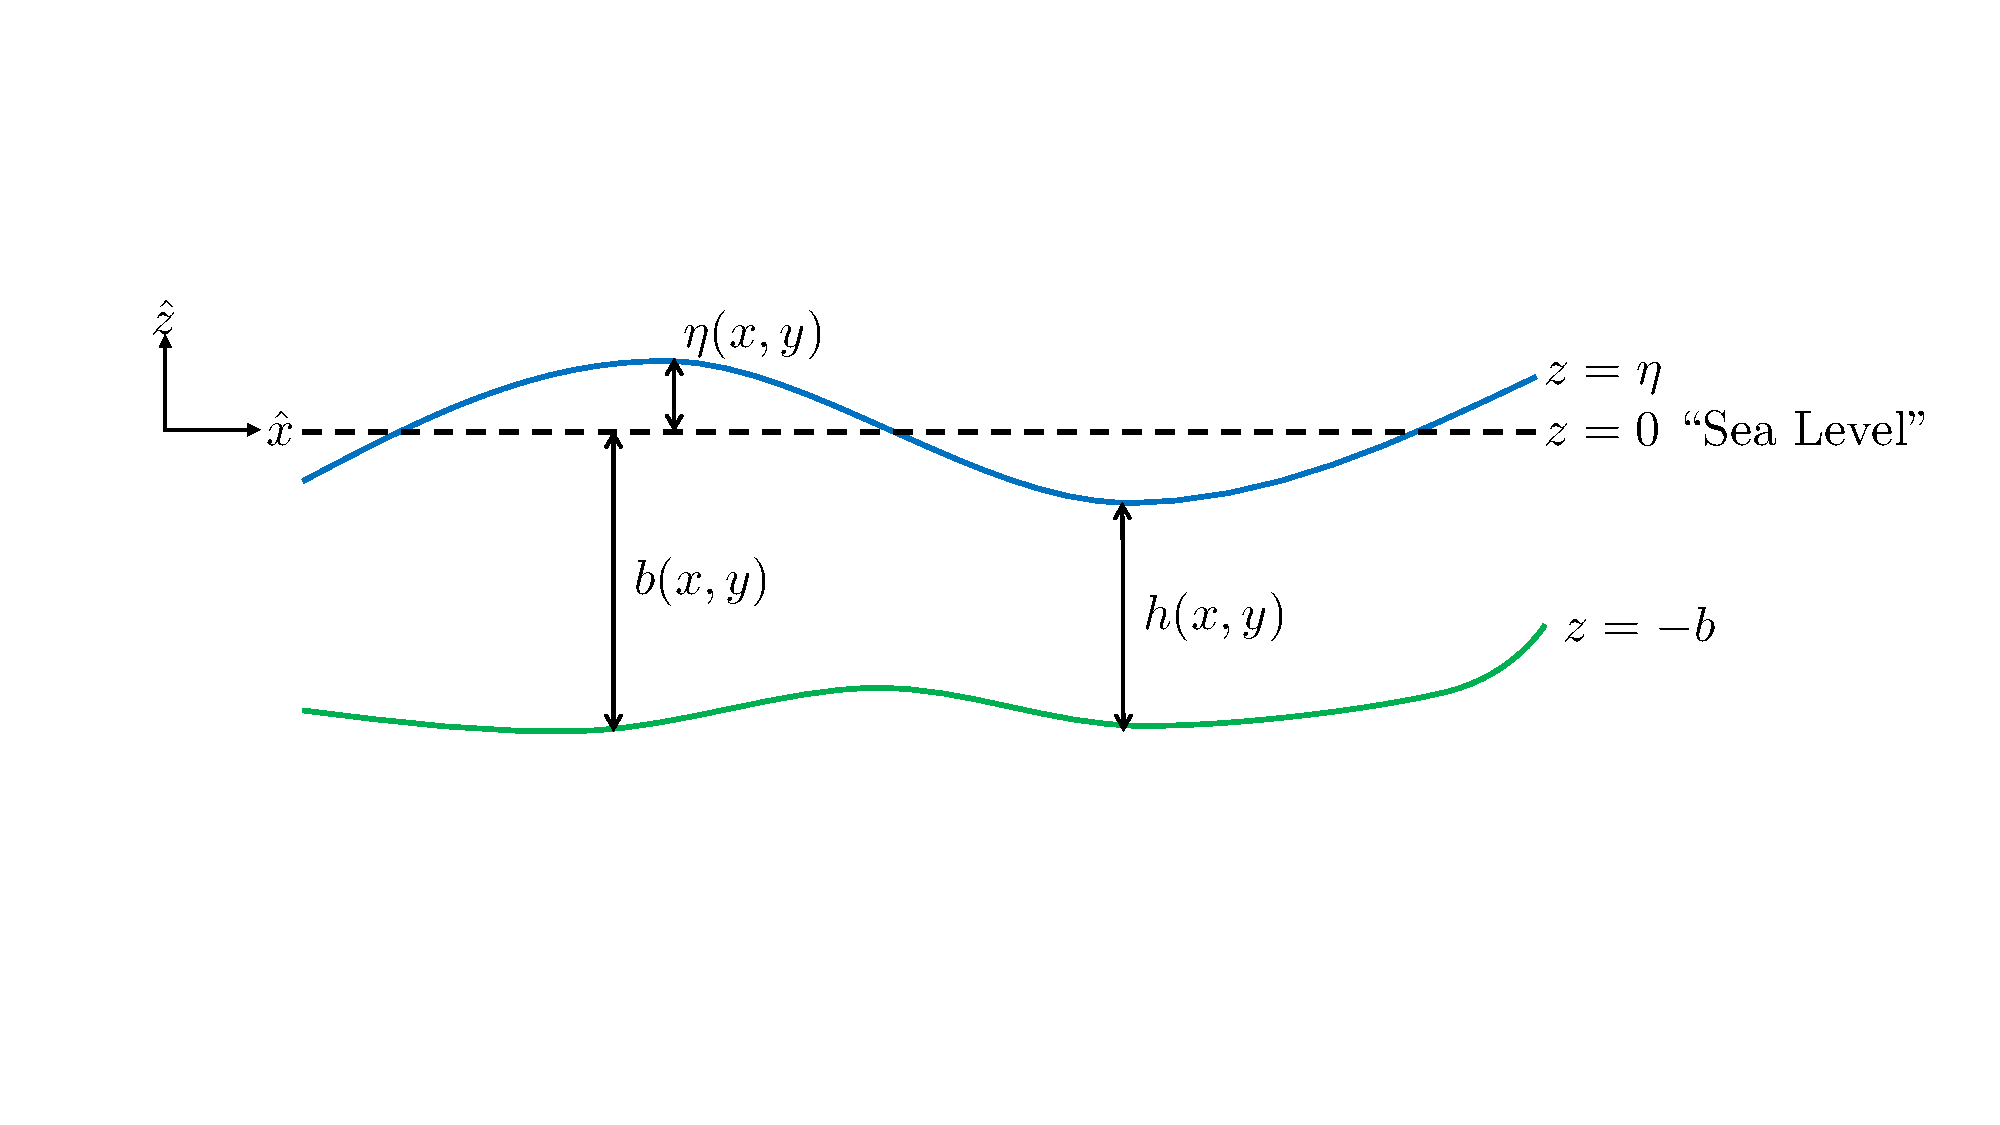
\includegraphics[width=\columnwidth]{figures/swe_model.pdf}
    \caption{Shallow Water Equaion Reference}
    \label{fig_swe}
\end{figure}

Various improvements have been made to the shallow water model in order to account for more accurate physics. These developments include adding a dispersive term correction to the model.

\subsection{Dispersive Term Correction}
\label{sec:dtc}

In the classical derivation of the shallow water equations, or the Saint-Venant system, the approach is to use a perturbation method to neglect any terms that are of the order of $\mathcal{O}(\mu)$, where
\begin{align}
\mu = \frac{h_0^2}{l^2}
\end{align}
is a parameter that describes the ``shallowness" of the fluid. For a shallow water regime, this would imply that $\mu \ll 1$.

In order to account for dispersive effects and generate a higher order system, Boussinesq in 1872 \cite{boussinesq1872theorie} also used perturbation theory, but included terms up to $\mathcal{O}(\mu^2)$. An additional contribution to this system by Peregrine \cite{peregrine1967long} considers variable depth (bathymetry). This leads to the following system expressed in non-dimensional form
\begin{align}
    \begin{cases}
        \frac{\partial \eta}{\partial t} + \nabla \cdot (h \textbf{u}) = 0 \\
        \frac{\partial \textbf{u}}{\partial t} + \epsilon (\textbf{u} \cdot \nabla \textbf{u}) + \nabla \eta = \mu \mathcal{D} + \mathcal{O}(\mu^2).
    \end{cases}
\label{boussinesq_model}
\end{align}
where $\mathcal{D}$ accounts for nonhydrostatic and dispersive effects, and is a function of $\eta$, $\textbf{u}$, and their derivatives. In Peregrine's derivation, $\mathcal{D}$ is expressed as
\begin{align}
\mathcal{D} = \frac{h}{2} \nabla \Big( \nabla \cdot \big( h \frac{\partial \textbf{u}}{\partial t} \big) \Big) - \frac{h^2}{6} \nabla^2 \Big( \frac{\partial \textbf{u}}{\partial t} \Big).
\end{align}

From this point, a group from France comprised of Lannes, Bonneton, Marche, Chazel, and Tissier develop addition theory and classes of nonlinear shallow water equation models in \cite{bonneton2011splitting}, \cite{lannes2009derivation}, and \cite{lannes2015new}. They stem from what are called the Serre-Green-Naghdi equations and they derive a modified Serre-Green-Nagdhi model that is more stable, dimensionally decoupled, and time-independent. This model is given below:
%
% % , and we will follow some of their derivations here. The derivations start with ``Boussinesq-type equations" (Lannes, et al.) and are cast into the Serre-Green-Naghdi equations. Then, they are improved upon twice, once with added frequency dispersion stability and further into a class of equations that are easier to solve numerically due to a time and state independent, diagonalized operator.
%
% \subsubsection{From Boussinesq to Serre-Green-Naghdi}
% \label{sub:b2sgn}
%
% In \cite{lannes2009derivation}, Lannes et al. start with the Boussinesq formulation in (\ref{boussinesq_model}) and describe various other formulations that have been analyzed for this class of equations. This leads to the Serre-Green-Nagdhi equations, which arise from a higher order ($\mathcal{O}(\mu^2)$) perturbation analysis than performed in the derivation of the classical shallow water equations. The Serre-Green-Naghdi equations as derived in \cite{lannes2009derivation} are given in a cleaner form in \cite{bonneton2011splitting} as the following:
% \begin{align}
%     \begin{cases}
%         \frac{\partial \eta}{\partial t} + \nabla \cdot (h \textbf{u}) = 0 \\
%         \big( \textbf{I} + \mu \mathcal{T} \big) \frac{\partial \textbf{u}}{\partial t} + \nabla \eta + \epsilon(\textbf{u} \cdot \nabla) \textbf{u} + \epsilon \mu \mathcal{Q}(\textbf{u}) = 0
%     \end{cases}
% \label{sgn}
% \end{align}
% where the following operators are defined
% \begin{align}
% \mathcal{T} [h, b] (\textbf{u}) &= \mathcal{R}_1 (\nabla \cdot \textbf{u}) + \beta \mathcal{R}_2 (\nabla b \cdot \textbf{u}), \\
% \mathcal{Q} [h, b] (\textbf{u}) &= \mathcal{R}_1 (\nabla \cdot (\textbf{u} \nabla \cdot \textbf{u}) - 2 (\nabla \cdot \textbf{u})^2) + \beta \mathcal{R}_2 ((\textbf{u} \cdot \nabla)^2 b) \\
% \mathcal{R}_1 [h,b] (w) &= -\frac{1}{3h} \nabla(h^3w) - \beta \frac{h}{2} w \nabla b \\
% \mathcal{R}_2 [h,b] (w) &= \frac{1}{2h} \nabla(h^2 w) + \beta w \nabla b.
% \end{align}
%
% \subsubsection{From Serre-Green-Naghdi to Modified Serre-Green-Nagdhi}
% \label{sub:sgn2msgn}
%
% Following this, in \cite{bonneton2011splitting}, Bonneton et al. recast this system into a more numerically stable form for frequency dispersion and use a splitting approach to split the numerical solution into a hyperbolic-like problem and an elliptic-like problem. The hyperbolic part (which describe the wave properties) can then be solved via high-order finite volume methods, and the elliptic part (which describe the dispersive properties) can be solved with a finite difference approach.
%
% In order to perform this splitting method, Bonneton et al. do the following: 1) Add other order $\mathcal{O}(\mu^2)$ terms to the momentum equation with a tuning parameter $\alpha$ to improve the frequency dispersion. Their logic in doing so is because the scheme is already precise up to terms of order $\mathcal{O}(\mu^2)$, ``this manipulation does not affect the precision of the model" (Bonneton et al.). And 2) reformulate $\eta$ and $\textbf{u}$ into $h$ and $h \textbf{u}$ in such a way that allows them to factor out terms that reduce the 3rd order derivatives into 2nd order. This makes the scheme less numerically stiff.
%
% Following these steps, Bonneton et al. arrive at the following modified Serre-Green-Nagdhi equations:
%
% \begin{align}
%     \begin{cases}
%         \frac{\partial h}{\partial t} + \nabla \cdot (h \textbf{u}) = 0 \\
%         \big[ \textbf{I} + \alpha \textbf{T} \big] \big[ \frac{\partial}{\partial t} (h \textbf{u}) + \frac{\alpha - 1}{\alpha} g h \nabla \eta + \nabla \cdot (h \textbf{u} \otimes \textbf{u}) \big] + \frac{1}{\alpha} g h \nabla \eta + h \mathcal{Q}_1(\textbf{u}) = 0
%     \end{cases}
% \label{msgn}
% \end{align}
% where the linear operator $\mathcal{Q}_1$ is:
% \begin{align}
% \mathcal{Q}_1 [h,b] (\textbf{u}) &= -2 \mathcal{R}_1(\frac{\partial \textbf{u}}{\partial x} \cdot \frac{\partial \textbf{u}}{\partial y} + (\nabla \cdot \textbf{u})^2) + \beta \mathcal{R}_2(\textbf{u} \cdot (\textbf{u} \cdot \nabla) \nabla b)
% \end{align}
% and
% \begin{align}
% \textbf{T} \textbf{w} = h \mathcal{T} \big( \frac{1}{h} \textbf{w} \big)
% \end{align}
%
% Upon observation, we notice that there are new terms compared to (\ref{sgn}) with the parameter $\alpha$ which acts as a tuning parameter for the frequency dispersion and is choosen to enable stability (more on this in the next section). Additionally, we notice that this model effectively decouples the wave propagation (the first three terms in the momentum equation) and the dispersion effects (the last two terms). This split model is ideal for coupling hyperbolic and elliptic solvers.
%
% It is these equations that Popinet uses in \cite{popinet2015quadtree} to develop a quadtree-adaptive multigrid solver to solve the SGN equations. In their approach, they cast (\ref{msgn}) into a system of conservation laws (hyperbolic system), where the dispersion terms appear in the source terms. The dispersive source terms are solved for by solving an elliptic-like equation that involve inverting the operator $\textbf{I} + \alpha h \mathcal{T} \frac{1}{h})$. Their approach is to use a multigrid method to solve for the dispersive terms. We will expand on this elliptic solve in the later sections.
%
% \subsubsection{From Modified Serre-Green-Nagdhi to Constant-Diagonal Serre-Green-Nagdhi}
%
% Now, the matrix operator $\textbf{T}$ has the form
% \begin{align}
% \textbf{T} =
% \begin{bmatrix}
%     \mathcal{T}_{11} & \mathcal{T}_{12} \\
%     \mathcal{T}_{21} & \mathcal{T}_{22} \\
% \end{bmatrix}
% \end{align}
% where $\mathcal{T}_{ij}$ are second order scalar differential operators. In order to solve for the dispersive terms in the models given, one needs to invert this operator, and the fact that $\textbf{T}$ has nonzero off-diagonals makes inverting this operator difficult; it couples together the disersive terms in both the x- and y-directions. Furthermore, each scalar operator $\mathcal{T}_{ij}$ is state dependent. This means that $\textbf{T}$ changes each time step in the hyperbolic system. Thus, in \cite{lannes2015new} Lannes et al. recast the modified Serre-Green-Nagdhi model into a constant-diagonal Serre-Green-Nagdhi model which eliminates the off-diagonal entries in $\textbf{T}$ and shifts the state dependency to a term outside the operator inversion.
%
% Lannes et al. do this in two steps. First, working in non-dimensional variables, they cast the momemtum equation from (\ref{msgn})
%
% \begin{align}
% (\textbf{I} + \mu \textbf{T}) \big[ \frac{\partial \textbf{u}}{\partial t} + \epsilon (\textbf{u} \cdot \nabla) \textbf{u} \big] + \nabla \eta + \epsilon \mu \mathcal{Q}_1(\textbf{u}) &= 0
% \end{align}
% into the form
% \begin{align}
% (\textbf{I} + \mu \textbf{T}_{diag}) \big[ \frac{\partial \textbf{u}}{\partial t} + \epsilon (\textbf{u} \cdot \nabla) \textbf{u} \big] + \nabla \eta + \epsilon \mu \mathcal{Q}_1(\textbf{u}) + \mu \mathcal{Q}_2(\eta) &= 0
% \label{dsgn}
% \end{align}
% where $\textbf{T}_{diag}$ has a diagonal structure. The goal is to now derive an expression for $\mathcal{Q}_2$ that permits the transformation. This is essentially done by applying the operator $\mathcal{T}$ to the acceleration and advection terms ($\partial_t \textbf{u}$ and $\epsilon (\textbf{u} \cdot \nabla) \textbf{u}$) and solving for the missing terms that need to appear in $\mathcal{Q}_2$ to maintain equality. This leads to
% \begin{align}
% \mathcal{Q}_2 (\eta) &= -h (\nabla^{\bot} h \cdot \nabla) \nabla^{\bot} \eta - \frac{\beta}{2h} \nabla(h^2 \nabla b \cdot \nabla \eta) + \beta \big(\frac{h}{2} \nabla^2 \eta - \beta (\nabla b \cdot \nabla \eta) \big) \nabla b
% \end{align}
% where $\nabla^{\bot} = (-\partial_y, \partial_x)^{T}$.
%
% Second, to eliminate the time dependency of the operator $\textbf{I} + \mu \textbf{T}_{diag}$, Lannes et al. perform a change of reference in order to cast $h$ as $h_b$, where $h_b$ is the water depth at rest and given by
% \begin{align}
% h_b = 1 - \beta b = h - \epsilon \eta
% \end{align}
% This allows them to write the matrix operator as
% \begin{align}
% \textbf{T}_{diag}^b = h_b \mathcal{T}_{diag}^b \frac{1}{h_b}
% \end{align}
% with
% \begin{align}
% \mathcal{T}_{diag}^b = -\frac{1}{3h_b} \frac{\partial}{\partial x} (h_b^3 \frac{\partial}{\partial x} \cdot) - \frac{1}{3 h_b} \frac{\partial}{\partial y} (h_b^3 \frac{\partial}{\partial y} \cdot)
% \end{align}
%
% In order to include this time independent matrix operator in the momentum, Lannes et al. formulate the following: For a scalar function $f$
%
% \begin{align}
% h \mathcal{T}_{diag} \frac{1}{h} f = h_b \mathcal{T}_{diag}^b \frac{1}{h_b} f + \mathcal{S} [h^2 - h^2_b] f
% \end{align}
% with
% \begin{align}
% \mathcal{S}[h^2 - h^2_b] f = -\frac{1}{6} \nabla(h^2 - h^2_b) \cdot \nabla f - \frac{h^2 - h^2_b}{3} \nabla^2 f + \frac{1}{6} \nabla^2 (h^2 - h^2_b) f.
% \end{align}
%
% Rewriting (\ref{dsgn}) with $\textbf{T}_{diag}^b$ and using the expressions above to account for the change lead to the constant-diagonal Serre-Green-Naghdi model
%
% \begin{align}
%     \begin{cases}
%         \frac{\partial h}{\partial t} + \epsilon \nabla \cdot (h \textbf{u}) = 0 \\
%         \big[ \textbf{I} + \mu \textbf{T}_{diag}^b \big] \big[ \frac{\partial}{\partial t} (h \textbf{u}) + \epsilon \nabla \cdot (h \textbf{u} \otimes \textbf{u}) \big] + ... \\
%         ... + h \nabla \eta + \epsilon \mu h \mathcal{Q}_1(\textbf{u}) + \mu h \mathcal{Q}_2 (\eta) + \mu \mathcal{Q}_3 (\eta) = 0
%     \end{cases}
%     \label{cdsgn}
% \end{align}
% where
% \begin{align}
%     \mathcal{Q}_3 (\eta) = -\mathcal{S}[h^2 - h^2_b] [\textbf{I} + \mu \textbf{T}_{diag}^b]^{-1} (h \nabla \eta).
% \end{align}
%
% This final expression gives the Serre-Green-Naghdi model in a form that decouples the x- and y-component, is time and state independent, is numerically stable, and is asymptotically accurate for order $\mathcal{O}(\mu^2)$ dispersion terms. A quick observation from (\ref{cdsgn}): if we neglect any order $\mathcal{O}(\mu)$ terms, we arrive at the classic Saint-Venant system of shallow water equations derived in \ref{sec:dswe}.
%
% In \cite{lannes2015new} Lannes et al. use von Neumann stability analysis to develop expressions for $\alpha$ for this model and for the classic Serre-Green-Naghdi model. They show that their new model is also stable for certain criteria for $\alpha$, namely $\alpha \ge 1$. For their modeling in \cite{lannes2015new}, they choose $\alpha = 1.159$.
%
% As a summary, we list all the parameters introduced in this derivation below:
%
% \begin{align*}
%     \epsilon &= \frac{a}{h_0} = \text{Nonlinearity Parameter} \\
%     \mu &= \frac{h_0^2}{L^2} = \text{Shallowness Parameter} \\
%     \beta &= \frac{a_{bottom}}{h_0} = \text{Topology Variation Parameter} \\
%     a &= \text{Typical Amplitude of Waves} \\
%     a_{bottom} &= \text{Typical Amplitude of bathymetry} \\
%     L &= \text{Order of Wavelength of Waves} \\
%     h_0 &= \text{Reference Depth} \\
%     \alpha &= \text{Frequency Tuning Parameter}
% \end{align*}
%
% \subsection{Towards Solving the Serre-Green-Nagdhi Model}
% \label{sec:tstsgnm}
%
% As a final step in this derivation, we motivate the solution methodology presented in the next chapter by casting the constant-diagonal SGN model into it's dimensional version and show how to split the problem into a hyperbolic problem and an elliptic one. This will put the model into a form similar to the form used by Popinet in \cite{popinet2015quadtree}, but with a slightly modified dispersion term to account for the adjustment from the modified SGN model to the constant-diagonal SGN model.
%
% The constant-diagonal SGN model is given below in it's dimensional version

\begin{align}
    \begin{cases}
        \frac{\partial h}{\partial t} + \nabla \cdot (h \textbf{u}) = 0 \\
        \frac{\partial}{\partial t} (h \textbf{u}) + \nabla \cdot (h \textbf{u} \otimes \textbf{u}) + \frac{\alpha - 1}{\alpha} g h \nabla \eta + \textbf{d} = 0
    \end{cases}
    \label{dcdsgn}
\end{align}
where $\textbf{d}$ is the solution of the following
\begin{align}
    \big( \textbf{I} + \alpha \textbf{T}_{diag}^b \big) \textbf{d} = \frac{gh}{\alpha} \nabla \eta + h\big( \mathcal{Q}_1(\textbf{u}) + g \mathcal{Q}_2(\eta) \big) + g \mathcal{Q}_3 (\eta)
    \label{eq4d}
\end{align}
and the dispersion matrix being
\begin{align}
    \textbf{T}_{diag}^b =
    \begin{bmatrix}
        \mathcal{T}_{diag}^b & 0 \\
        0 & \mathcal{T}_{diag}^b \\
    \end{bmatrix}
\end{align}
and the operators are given in their dimensional versions as
\begin{align}
    \mathcal{T}_{diag}^b &= -\frac{1}{3 h_b} \frac{\partial}{\partial x}\big( h_b^3 \frac{\partial}{\partial x} \big) - \frac{1}{3 h_b} \frac{\partial}{\partial y}\big( h_b^3 \frac{\partial}{\partial y} \big) \\
    \mathcal{Q}_1 [h,b] (\textbf{w}) &= -2 \mathcal{R}_1(\frac{\partial \textbf{w}}{\partial x} \cdot \frac{\partial \textbf{w}}{\partial y} + (\nabla \cdot \textbf{w})^2) + \beta \mathcal{R}_2(\textbf{w} \cdot (\textbf{w} \cdot \nabla) \nabla b) \\
    \mathcal{Q}_2 [h,b] (\eta) &= -h (\nabla^{\bot} h \cdot \nabla) \nabla^{\bot} \eta - \frac{\beta}{2h} \nabla(h^2 \nabla b \cdot \nabla \eta) + \beta \big(\frac{h}{2} \nabla^2 \eta - \beta (\nabla b \cdot \nabla \eta) \big) \nabla b \\
    \mathcal{Q}_3 [h,b] (\eta) &= -\mathcal{S}[h^2 - h^2_b] [\textbf{I} + \mu \textbf{T}_{diag}^b]^{-1} (h \nabla \eta) \\
    \mathcal{R}_1 [h,b] (w) &= -\frac{1}{3h} \nabla(h^3w) - \beta \frac{h}{2} w \nabla b \\
    \mathcal{R}_2 [h,b] (w) &= \frac{1}{2h} \nabla(h^2 w) + \beta w \nabla b \\
    \mathcal{S}[h^2 - h^2_b] f &= -\frac{1}{6} \nabla(h^2 - h^2_b) \cdot \nabla f - \frac{h^2 - h^2_b}{3} \nabla^2 f + \frac{1}{6} \nabla^2 (h^2 - h^2_b) f.
\end{align}
The parameters mentioned are summarized below:
\begin{align*}
    \mu &= \frac{h_0^2}{L^2} = \text{Shallowness Parameter} \\
    \beta &= \frac{a_{bottom}}{h_0} = \text{Topology Variation Parameter} \\
    a &= \text{Typical Amplitude of Waves} \\
    a_{bottom} &= \text{Typical Amplitude of bathymetry} \\
    L &= \text{Order of Wavelength of Waves} \\
    h_0 &= \text{Reference Depth} \\
    \alpha &= \text{Frequency Tuning Parameter}
\end{align*}

By integrating both equations in (\ref{dcdsgn}) over the domain, and using the divergence theorem on the second term in both equations, we arrive at the following integral formulation of the modified Serre-Green-Nagdhi model

\begin{align}
    \frac{\partial}{\partial t} \int_{\Omega} \textbf{q} d\Omega + \int_{\partial \Omega} \textbf{F}(\textbf{q}) \cdot \hat{\textbf{n}} d\partial \Omega + \int_{\Omega} \textbf{s} d\Omega = 0
\end{align}
where
\begin{align}
    \textbf{q} =
    \begin{bmatrix}
        h \\
        h u \\
        h v \\
    \end{bmatrix}\ \ \
    \textbf{F}(\textbf{q}) =
    \begin{bmatrix}
        h u & h v \\
        h u^2 + \frac{1}{2} g h^2 & h u v \\
        h u v & h u^2 + \frac{1}{2} g h^2 \\
    \end{bmatrix}\ \ \
    \textbf{s} =
    \begin{bmatrix}
        0 \\
        \frac{\alpha - 1}{\alpha} g h \frac{\partial \eta}{\partial x} + d_x \\
        \frac{\alpha - 1}{\alpha} g h \frac{\partial \eta}{\partial y} + d_y \\
    \end{bmatrix}.
\end{align}
This hyperbolic system can be solved using any standard approach to solving hyperbolic systems. The dispersive terms included in the source term need to be solved for through an elliptic solve. Each time step, one can call a solver in order to get the components of $\textbf{d}$. The elliptic expression (\ref{eq4d}) must be solved seperately from the hyperbolic each time step. Thus, in order to solve for $\textbf{d}$, we need to look at methods to solve elliptic systems. This motivates our next discussion and the content of the rest of this paper.

%%% Local Variables:
%%% mode: latex
%%% TeX-master: "BSUmain"
%%% End:
